\documentclass[9pt,twocolumn]{scrartcl}

%\documentclass[9pt]{sigcomm-alternate}

%\usepackage[margin=1in,bottom=1.2in]{geometry}
\usepackage{amsfonts,amssymb,amsmath}
\usepackage[thmmarks,hyperref,amsthm,amsmath]{ntheorem}
\usepackage{graphicx}
\usepackage[ruled,vlined,commentsnumbered]{algorithm2e}
\usepackage[usenames,dvipsnames]{color}
\usepackage{hyperref}
\usepackage{multirow}
\usepackage{lineno}
\usepackage[shortlabels]{enumitem}
\usepackage[utf8]{inputenc}
\usepackage[OT4]{fontenc}
\usepackage{comment}
\usepackage{fancyhdr}
\usepackage{tikz}
%Used Symbols
%c_i = chunk i
%v_i = vm i
%b_t = transfer bandwidth
%b_c = pairwise communication bandwidth
%n = |VMs| = |Chunks|


%Header Extensions Seperation
%Carlo
\newcommand{\VM}{\textsc{VM}}
\newcommand{\Chunk}{\textsc{chunk}}
\newcommand{\Problem}{\textsc{DummyName Problem}}
\newcommand{\carlo}[1]{\textcolor{red}{#1}}
\newcommand{\MaFactor}{\ensuremath{\textsc{MA}}} 


\newcommand{\VirtualNodes}{\ensuremath{V_V}}
\newcommand{\VirtualEdges}{\ensuremath{E_V}}
\newcommand{\VirtualNode}{\ensuremath{v}}
\newcommand{\VirtualEdge}{\ensuremath{e}}
\newcommand{\VCSwitch}{\ensuremath{\textsc{center}}}
\newcommand{\SubstrateNodes}{\ensuremath{V_S}}
\newcommand{\SubstrateEdges}{\ensuremath{E_S}}
\newcommand{\SubstrateNode}{\ensuremath{v}}
\newcommand{\SubstrateEdge}{\ensuremath{e}}
\newcommand{\Leaf}{\ensuremath{l}}
\newcommand{\Leaves}{\ensuremath{L}}


\newcommand{\VC}{\textsc{VC}}
\newcommand{\CC}{\textsc{CC}}

\newcommand{\VE}{\textsc{VE}}
\newcommand{\FP}{\textsc{FP}}
\newcommand{\RS}{\textsc{RS}}
\newcommand{\BW}{\textsc{BW}}
\newcommand{\Cost}{\textsc{Cost}}

\newcommand{\MatchCost}{\textsc{MCost}}
\newcommand{\chunkOf}{\textsc{chunkOf}}


%Maciek

\newcommand{\Bandwidth}{\ensuremath{bw}}
\newcommand{\Tree}{\ensuremath{T}}
\newcommand{\CostCom}{\ensuremath{b_1}}
\newcommand{\CostTrans}{\ensuremath{b_2}}
\newcommand{\Vms}{\ensuremath{VM}}


\newcommand{\Formula}{\ensuremath{\Psi}}
\newcommand{\Clauses}{\ensuremath{Cl(\Formula)}}
\newcommand{\NClauses}{\ensuremath{c}}
\newcommand{\Vars}{\ensuremath{Var(\Formula)}}
\newcommand{\NVars}{\ensuremath{|\Vars|}}
\newcommand{\ChunkTypes}{\ensuremath{ch}}
\newcommand{\Thr}{\ensuremath{Th}}
\newcommand{\VCB}{\ensuremath{VCB}}
\newcommand{\VCNB}{\ensuremath{VCNB}}
\newcommand{\varx}{\ensuremath{x}}
\newcommand{\positive}{\ensuremath{positive}}
\newcommand{\negative}{\ensuremath{negative}}
\newcommand{\SAT}{\ensuremath{SAT}}
\newcommand{\TSAT}{\ensuremath{3SAT}}
\newcommand{\Val}{\ensuremath{Val}}
\newcommand{\Sol}{\ensuremath{SOL}}



\definecolor{blueLink}{rgb}{0,0.2,0.8}
\hypersetup{colorlinks,linkcolor=blueLink,urlcolor=blueLink,citecolor=blueLink}
\newcommand{\lref}[2][]{\hyperref[#2]{#1~\ref*{#2}}}



%%%%%%%%%%%%%%%%%%%%%%%%%%%%%%%%%%%%%%%%%%%%%%%%%%%%%%%%%%%%%
% GENERAL STYLE MACROS
%%%%%%%%%%%%%%%%%%%%%%%%%%%%%%%%%%%%%%%%%%%%%%%%%%%%%%%%%%%%%

\newcommand{\etal}{{\it et~al.\ }}
\newcommand{\myparagraph}[1]{{\smallskip\noindent{\bf #1}}}
\newcommand{\mycase}[1]{{\underline{Case~#1}:}}

%%%%%%%%%%%%%%%%%%%%%%%%%%%%%%%%%%%%%%%%%%%%%%%%%%%%%%%%%%%%
% THEOREMS AND SUCH
%%%%%%%%%%%%%%%%%%%%%%%%%%%%%%%%%%%%%%%%%%%%%%%%%%%%%%%%%%%%%

\newtheorem{theorem}{Theorem}
\newtheorem{corollary}[theorem]{Corollary}
\newtheorem{lemma}[theorem]{Lemma}
\newtheorem{claim}[theorem]{Claim}
\newtheorem{fact}{Fact}

%%%%%%%%%%%%%%%%%%%%%%%%%%%%%%%%%%%%%%%%%%%%%%%%%%%%%%%%%%%%%
% USEFUL LETTERS
%%%%%%%%%%%%%%%%%%%%%%%%%%%%%%%%%%%%%%%%%%%%%%%%%%%%%%%%%%%%%

\DeclareMathOperator{\polylog}{polylog}
\newcommand{\emdash}{\hspace{1mm}---\hspace{1mm}}
\newcommand{\e}{\mathrm{e}}
\renewcommand{\O}{\mathcal{O}}
\renewcommand{\Pr}{\mathbf{Pr}}
\newcommand{\E}{\mathbf{E}}
\newcommand{\NAT}{\mathbb{N}}
\newcommand{\REAL}{\mathbb{R}}

%%%%%%%%%%%%%%%%%%%%%%%%%%%%%%%%%%%%%%%%%%%%%%%%%%%%%%%%%%%%%
% PARENTHESES ETC
%%%%%%%%%%%%%%%%%%%%%%%%%%%%%%%%%%%%%%%%%%%%%%%%%%%%%%%%%%%%%

\newcommand{\ceiling}[1]{\left\lceil #1 \right\rceil}
\newcommand{\floor}[1]{\left\lfloor #1 \right\rfloor}
\newcommand{\braced}[1]{{\left\{#1\right\}}}
\newcommand{\bigbrackd}[1]{{\big[#1\big]}}
\newcommand{\brackd}[1]{{\left[#1\right]}}
\newcommand{\parend}[1]{{\left(#1\right)}}

%%%%%%%%%%%%%%%%%%%%%%%%%%%%%%%%%%%%%%%%%%%%%%%%%%%%%%%%%%%%%
% FRACTIONS
%%%%%%%%%%%%%%%%%%%%%%%%%%%%%%%%%%%%%%%%%%%%%%%%%%%%%%%%%%%%%

\newcommand{\half}{\frac{1}{2}}
\newcommand{\onehalf}{\frac{1}{2}}
\newcommand{\onethird}{\frac{1}{3}}
\newcommand{\twothirds}{{\textstyle\frac{2}{3}}}
\newcommand{\fourthirds}{{\textstyle\frac{4}{3}}}
\newcommand{\fivethirds}{{\textstyle\frac{5}{3}}}
\newcommand{\threefourths}{{\textstyle\frac{3}{4}}}

%%%%%%%%%%%%%%%%%%%%%%%%%%%%%%%%%%%%%%%%%%%%%%%%%%%%%%%%%%%%%
% ALGORITHM NAMES, ETC
%%%%%%%%%%%%%%%%%%%%%%%%%%%%%%%%%%%%%%%%%%%%%%%%%%%%%%%%%%%%%

\newcommand{\ALG}{\textsc{Alg}}
\newcommand{\OPT}{\textsc{Opt}}
\newcommand{\DET}{\textsc{Det}}
\newcommand{\RAND}{\textsc{Rand}}

%%%%%%%%%%%%%%%%%%%%%%%%%%%%%%%%%%%%%%%%%%%%%%%%%%%%%%%%%%%%%
% PSEUDOCODE
%%%%%%%%%%%%%%%%%%%%%%%%%%%%%%%%%%%%%%%%%%%%%%%%%%%%%%%%%%%%%

\newcommand{\IF}    {{\bf if }}
\newcommand{\THEN}  {{\bf then }} 
\newcommand{\FOR}   {{\bf for }}
\newcommand{\EACH}  {{\bf each }} 
\newcommand{\DO}  {{\bf do }} 

%%%%%%%%%%%%%%%%%%%%%%%%%%%%%%%%%%%%%%%%%%%%%%%%%%%%%%%%%%%%%
% EDITORIAL MACROS
%%%%%%%%%%%%%%%%%%%%%%%%%%%%%%%%%%%%%%%%%%%%%%%%%%%%%%%%%%%%%

\definecolor{brown}{rgb}{0.4,0,0} 
\definecolor{purple}{rgb}{0.2,0,0.6}
\definecolor{hotpink}{rgb}{1,0.4,0.7}
\newcommand{\marginnote}[1]{\marginpar{\scriptsize{\begin{flushleft}#1\end{flushleft}}}}
\newcommand{\todo}[1]{\noindent\colorbox{red}{todo: #1}} 
\newcommand{\marcin}[1]{\color{red} Marcin: #1\color{black}}



\title{A Note on Virtual Cluster Embedding with Data Locality}

\title{Embedding Algorithms for Virtual Clusters with Data Locality and Replica Selection}

\title{Embedding Virtual Clusters with Data Locality and Replica Selection\\{\Large Real Algorithms for Virtual Environments}}


\author{Maciek, Carlo, Stefan}

\begin{document}
\maketitle


\begin{abstract}
By decoupling applications from the constraints of the underlying physical
infrastructure, virtualization introduces a very flexible resource allocation model.
Accordingly, over the last years, many algorithms have been proposed to exploit
these flexibilities in order to embed applications more efficiently. Especially the
virtual network embedding problem has been studied intensively.

However, theoretical studies on the virtual network embedding so far miss two important aspects,
which we call the \emph{data locality constraint} and \emph{replica selection opportunity}:
data locality refers to the fact that the input to cloud applications such as MapReduce
is typically already stored  in the datacenter and the corresponding constraints need to be taken into account when embedding
the application; and replica selection refers to the fact that input is often stored redundantly, and
hence introduces further optimization opportunities.

This paper studies the fundamental algorithmic challenges resulting from data locality
and replica selection.
In particular, we decompose virtual network embedding problems with locality constraints
into four
main aspects: flexible virtual node placement ($\FP$), communication costs ($\CC$),
replica selection ($\RS$),
and bandwidth constraints $\BW$.

This paper shows that both $\FP$ and $\RS$ problems can often be solved optimally in polynomial time,
using dynamic programming and max-flow (for $\FP$) algorithms, as well as matching algorithms (for $\RS$).
However, we also show that jointly optimizing the $\FP$, $\CC$,
and $\RS$ is NP-hard under bandwidth constraints $\BW$.

We believe that our paper can provide the networking community with important insights into the
design of algorithms to exploit resource allocation flexibilities in virtual environments, as well as the fundamental (computational)
limitations of such optimizations.
\end{abstract}

%%%%%%%%%%%%%%%%%%%%%%%%%%%%%%%%%%%%%
\section{Introduction}

Server virtualization has revamped the server business over the last years,
and has radically changed the way we think about resource allocation in the Internet today.
Indeed, the success of cloud computing relies to a large extent on virtualization:
the possibility to allocate virtual machines flexibly and on-demand.

The virtualization trend now started to spill over to the network. It is well-known
that provisioning virtual machines is often not sufficient to guarantee a predictable performance
to cloud applications, as the interference in the underlying network can significantly delay the
execution.~\cite{talk-about} This is particularly the case in batch-processing jobs such as MapReduce, which consume
a considerable amount of bandwidth resources during their execution.~\cite{amazonbw}

A most prominent virtual network abstraction is the \emph{Virtual Cluster} $\VC(n,b)$:
the virtual cluster provides the abstraction of $n$ virtual machines connected to a logical
switch at (at least) bandwidth $b$ (essentially a Hose model).~\cite{oktopus}
In other words, the virtual cluster provides isolation guarantees over both resources,
the computation (the virtual machines) and bandwidth (the network).

The problem of how to efficiently and jointly map the nodes and links of a virtual cluster in a given datacenter is non-trivial,
and has been studied for several years now.~\cite{oktopus,proteus,secondnet} The problem is complicated further when taking into account
\emph{data locality issues}: usually the inputs to a cloud application (the so-called \emph{chunks})
are stored in a
distributed database in the datacenter, \emph{in a redundant manner}. The virtual machine mapping algorithm should take into account
the locations
of the problem inputs (the chunks and their replicas), in order to avoid unnecessary transmissions over the network.

In this paper, we are interested in the fundamental algorithmic problems raised by virtualized datacenters,
where virtual machines can be placed flexibly and input data is stored redundantly:
How to exploit the flexibility of mapping virtual machines and their interconnecting
network flexibly, in order to minimize the resource footprint of the application while providing
the requested resources (and hence performance guarantees)?
And how to take into account data locality and exploit
redundancy in the distributedly stored problem input (replica selection)?

\subsection{Model}

We distinguish between two fundamental new optimization problems introduced by virtualization:
The decoupling of applications from the underlying physical infrastructure introduces node placement flexibilities ($\FP$):
virtual machines can be mapped to arbitrary nodes in the physical network. Moreover,
network virtualization technology and software-defined networking allows for a flexible selection of data replicas ($\RS$):
the input to cloud applications, the chunks, are typically stored in a distributed database, in a redundant fashion.
The $\FP$ and $\RS$ flexibilities introduce interesting new opportunities for optimization.

Besides mapping virtual machines ($\FP$) and matching them to their replicas ($\RS$), there are typically two more
aspects to be taken into account: (1) embedding a minimal virtual cluster network ($\VC$) to interconnect the virtual machines with certain
bandwidth guarantees, (2) while taking into account bandwidth constraints ($\BW$).

More formally, we consider the following problem. We are given a substrate network $H=(V,E)$ (the ``host graph'') consisting of servers $V$
interconnected by links $E$; we assume that $H$ forms a typical fat-tree datacenter.~\cite{todo}
For ease of presentation, we will assume that each server can host one virtual machines. (All our algorithms can easily be generalized to
a scenario where servers can host multiple virtual machines.)
The substrate stores the application input: we assume that a set of chunks $C$ are distributed over $V$, and that chunks may be redundant,
allowing for replica selection $\RS$. Moreover, the links $E$ can come with bandwidth capacity constraints ($\BW$).

The cloud application is described in the form of a virtual cluster $\VC(n,b)$, connecting $n$ virtual machines at a minimal bandwidth $b$
to a logical switch: a Hose model. Each virtual machine needs to be mapped to exactly one server. Moreover, we assume that for each chunk
assigned to a given virtual machine, we need to allocate bandwidth $b'$.

We seek to optimize the \emph{resource footprint} of the virtual cluster embedding: the amount of network resources which need to be allocated
to connect the chunks to virtual machines (cost $b'$ each) as well as to interconnect the virtual machines (at bandwidth $b$). That is,
the cost function consists of a matching cost $\MatchCost$ and a virtual cluster interconnection cost $\CC$.
and we want to minimize:
$$
\Cost = \MatchCost + \CC
$$
\noindent where $\MatchCost = \sum_{v\in \VC(n,b)} b'\cdot \ell(v,\chunkOf(v))$ and
$\CC = \sum_{v_1,v_2\in \VC(n,b)} \ell(v_1,v_2)$, where $\chunkOf(v)$ denotes
the chunk to which $v$ is mapped and $\ell$ is the distance
between two locations in the datacenter.

Sometimes, we are only interested in the matching problem or virtual cluster embedding alone,
and will ignore the other cost component.




\subsection{Our Contributions}

This paper takes a closer look at the fundamental resource allocation problems
in virtual network environments, studying and distinguishing between flexibilities in virtual machine placements ($\FP$) and
replica selection ($\RS$), taking into account communication costs ($\CC$) and bandwidth constraints ($\BW$).

We make the following contributions.
\begin{enumerate}
\item We show that the virtual cluster embedding dyn prog and flow
\item We show that the other is matching
\item NP-hardness
\end{enumerate}



\subsection{Paper Organization}


%%%%%%%%%%%%%%%%%%%%%%%%%%%%%%%%%%%%%
\section{Algorithms}

%%%%%%%%%%%%%%%%%%%%%%%%%%%%%%%%%%%%%%%
\subsection{Model variants}
\section{Model}

This section describes our model. We will start by describing a simplistic
version of our model, and continue to introduce new properties until we reach
the full model.

\subsection{Symbols}

This is a dummy section to introduce the symbols used later...

\begin{description}
 \item [$\Tree$] the substrate tree with $\Tree = (\SubstrateNodes , \SubstrateEdges)$
 \item [$\SubstrateNodes$]  a set of nodes: $\{\SubstrateNode_1, \dots ,
\SubstrateNode_{|\SubstrateNodes|}\}$
 \item [$\SubstrateEdges$] a set of edges : $\{\SubstrateEdge_1, \dots ,
 \SubstrateEdge_{|\SubstrateEdge|}\}$ with $\SubstrateEdge_1 =
(\SubstrateNode_i, \SubstrateNode_j)$
 \item [$c_i$] A chunk of type $i$
 \item [$v_i$] The i-th $\VM$ of the request
 \item [$\VirtualNodes$] the set of virtual Nodes = $\{1,2,\dots,\VCSwitch\}$
 \item [$\VirtualEdges$] the set of virtual Edges, $e_{V1}$ connects $1 \in
\VirtualNodes$ with $\VCSwitch \in \VirtualNodes$.
 \item [$\hat f$] the maximal flow
 \item [$|\hat f|$] the value of the maximal flow


 \item [$\Bandwidth$] Bandwidth constraint of an edge
 \item [$\CostTrans$] cost of chunk transport
 \item [$\CostCom$] cost of chunk communication
 \item [$\Vms$] number of VMs to spawn
 \item [$\ChunkTypes$] number of chunk types placed in an instance
 \item [$\Formula$] a formula
 \item [$\Clauses$] set of clauses in a formula
 \item [$\NClauses$] number of clauses in a given formula
 \item [$\Vars$] set of variables in a given formula
 \item [$\NVars$] number of variables in a given formula
 \item [$\Thr$] threshold
 \item [$\VCB$] virtual cluster model with bandwith
 \item [$\VCNB$] virtual cluster model without bandwith
 \item [$\varx$] variable
 \item [$\positive$] positive subtree of a gadget
 \item [$\negative$] negative subtree of a gadget
 \item [$\SAT$] set of satisfiable boolean formulas in CNF
 \item [$\TSAT$] set of satisfiable boolean formulas in 3CNF
 \item [$\Val$] valuation
 \item [$\Sol$] soultion to VC instance

\end{description}



\subsection{The Basic Model}

\carlo{Section TODO: How many / which figures + order?}

In the basic version of $\Problem$ data in the form of multiple chunks is
located in an undirected host graph tree $\Tree = (\SubstrateNodes,
\SubstrateEdges)$. A chunk $\Chunk$ of the set of chunks $\Chunks =
\{\Chunk_1,\dots,\Chunk_{\ChunkTypes}\}$ can only be located at the leaves
$\Leaves = \{\Leaf_1,\dots,\Leaf_m\} \subset \SubstrateNodes$ of $\Tree$. We
denote the location of a chunk by $\ChunkLocation : \Chunks \rightarrow
\Leaves$. A cluster, consisting of a set of VMs $\VirtualNodes =
\{\VirtualNode_1,\dots,\VirtualNode_{\Vms}\}$, is allready embedded on the host
graph, and should process this data. The VMs are embedded on the
leaves of the tree, and we denote the location of the VMs by $\NodeMapping :
\VirtualNodes \rightarrow \Leaves$. We assume that $\Vms = \ChunkTypes$, each
VM $\VirtualNode_i$ can read the data of one chunk $\Chunk_j$, and the data of
each chunk $\Chunk_j \in \Chunks$ has to be processed. In order to process the
data from a chunk $\Chunk_j$ with the VM $\VirtualNode_i$ it has to be
transferred along a (potentially empty) path $\Path_j =
\{\SubstrateEdge_{j_1},\dots,\SubstrateEdge_{j_n}\} ~ \SubstrateEdge_{j_k} \in
\SubstrateEdges$ such that $\SubstrateEdge_{j_1} = (\ChunkLocation(\Chunk_j),
\SubstrateNode_x)$, $\SubstrateEdge_{j_k} = (\SubstrateNode_x,
\SubstrateNode_y) \rightarrow \SubstrateEdge_{j_{k+1}} = (\SubstrateNode_y ,
\SubstrateNode_z)$, and $\SubstrateEdge_n = (\SubstrateNode_y,
\NodeMapping(\VirtualNode_i))$.  For the sake of simplicity we assume that
transferring a chunk over a link in the host graph inflicts bandwidth cost of
$\CostTrans$ on this link. The overall objective of $\Problem$ is to find an
assignment of VMs to chunks $\VmChunkAssignment : \Chunks \rightarrow
\SubstrateNodes$, so that the overall costs $\sum_{j \in
\{1,\dots,\ChunkTypes\}} |\Path_j|$ are minimized.

\begin{figure}

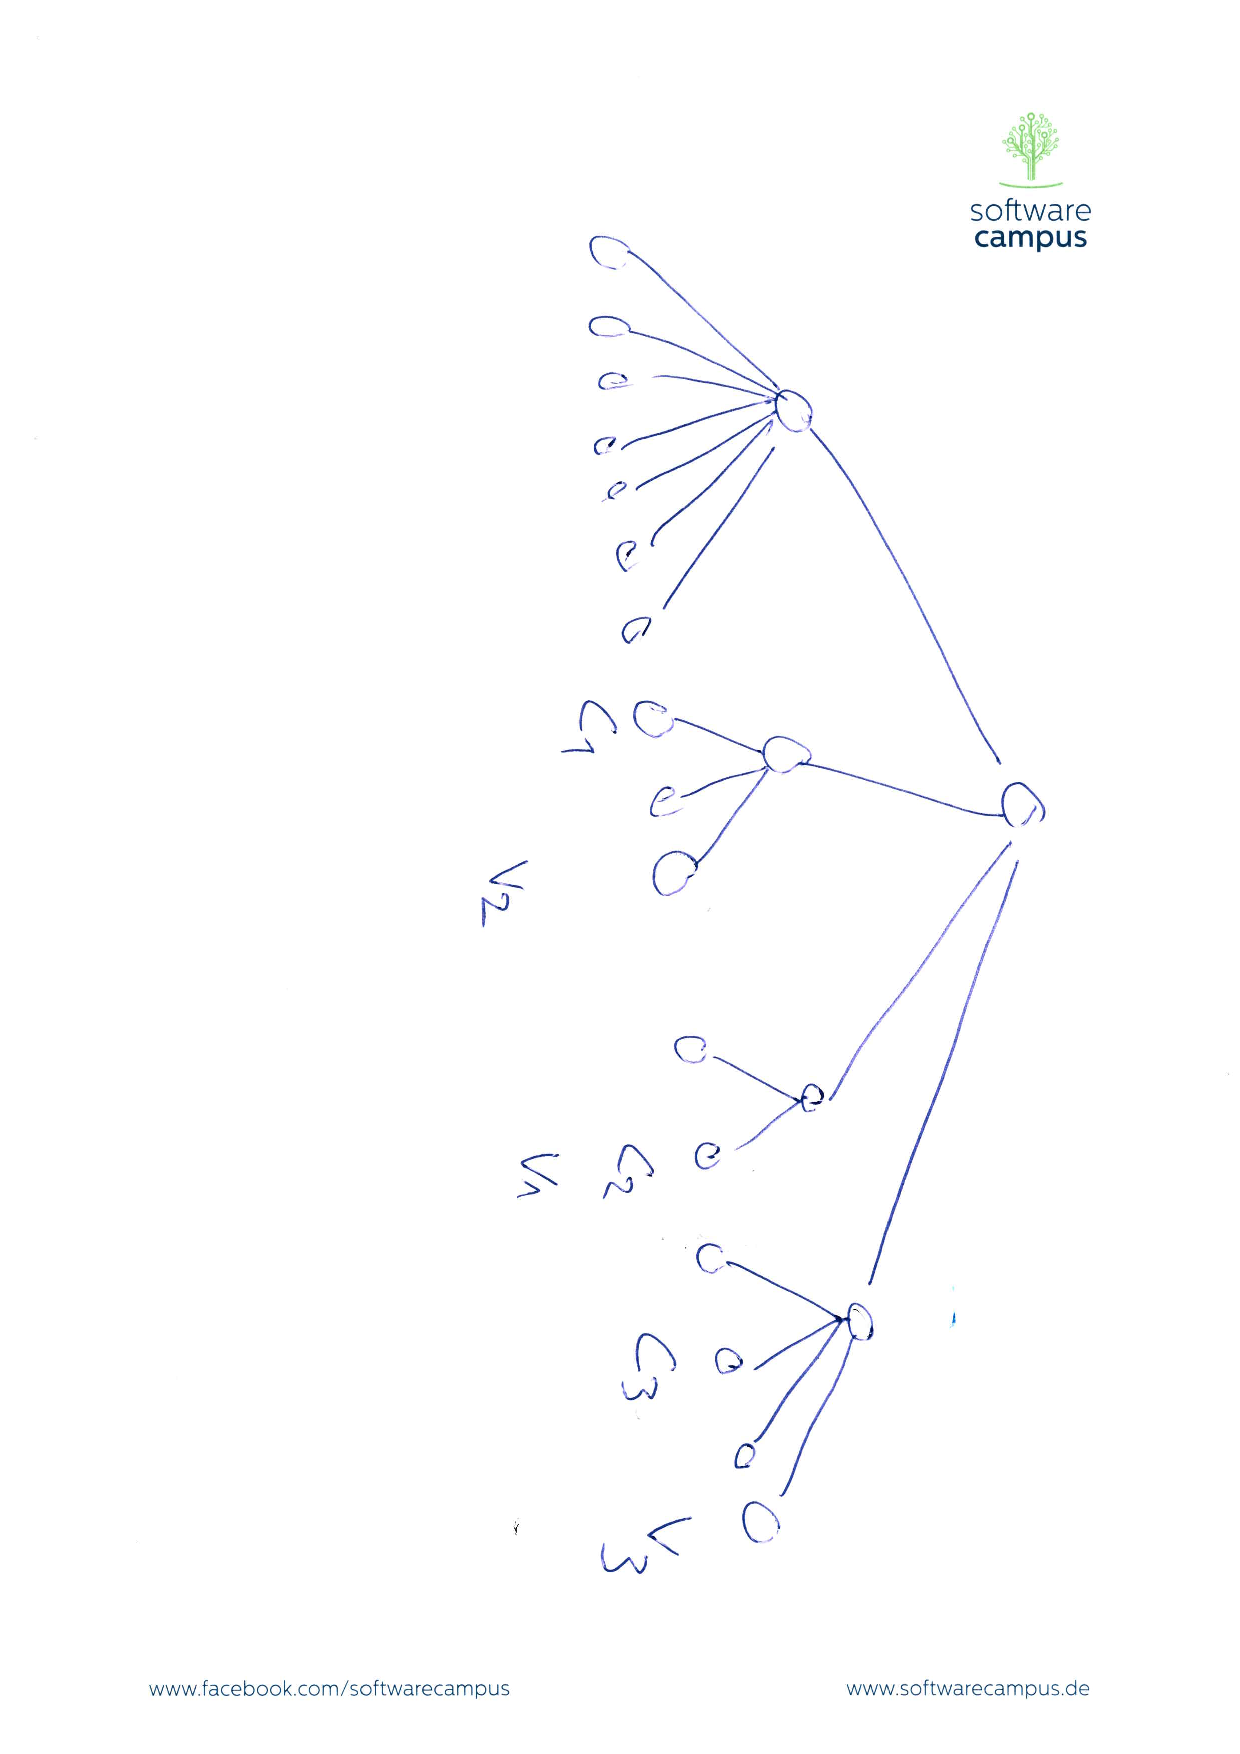
\includegraphics[angle=90,origin=c, height=7cm]{figs/model_fig_skteches/basic_problem}
\caption{basic problem}
\end{figure}
\begin{figure}

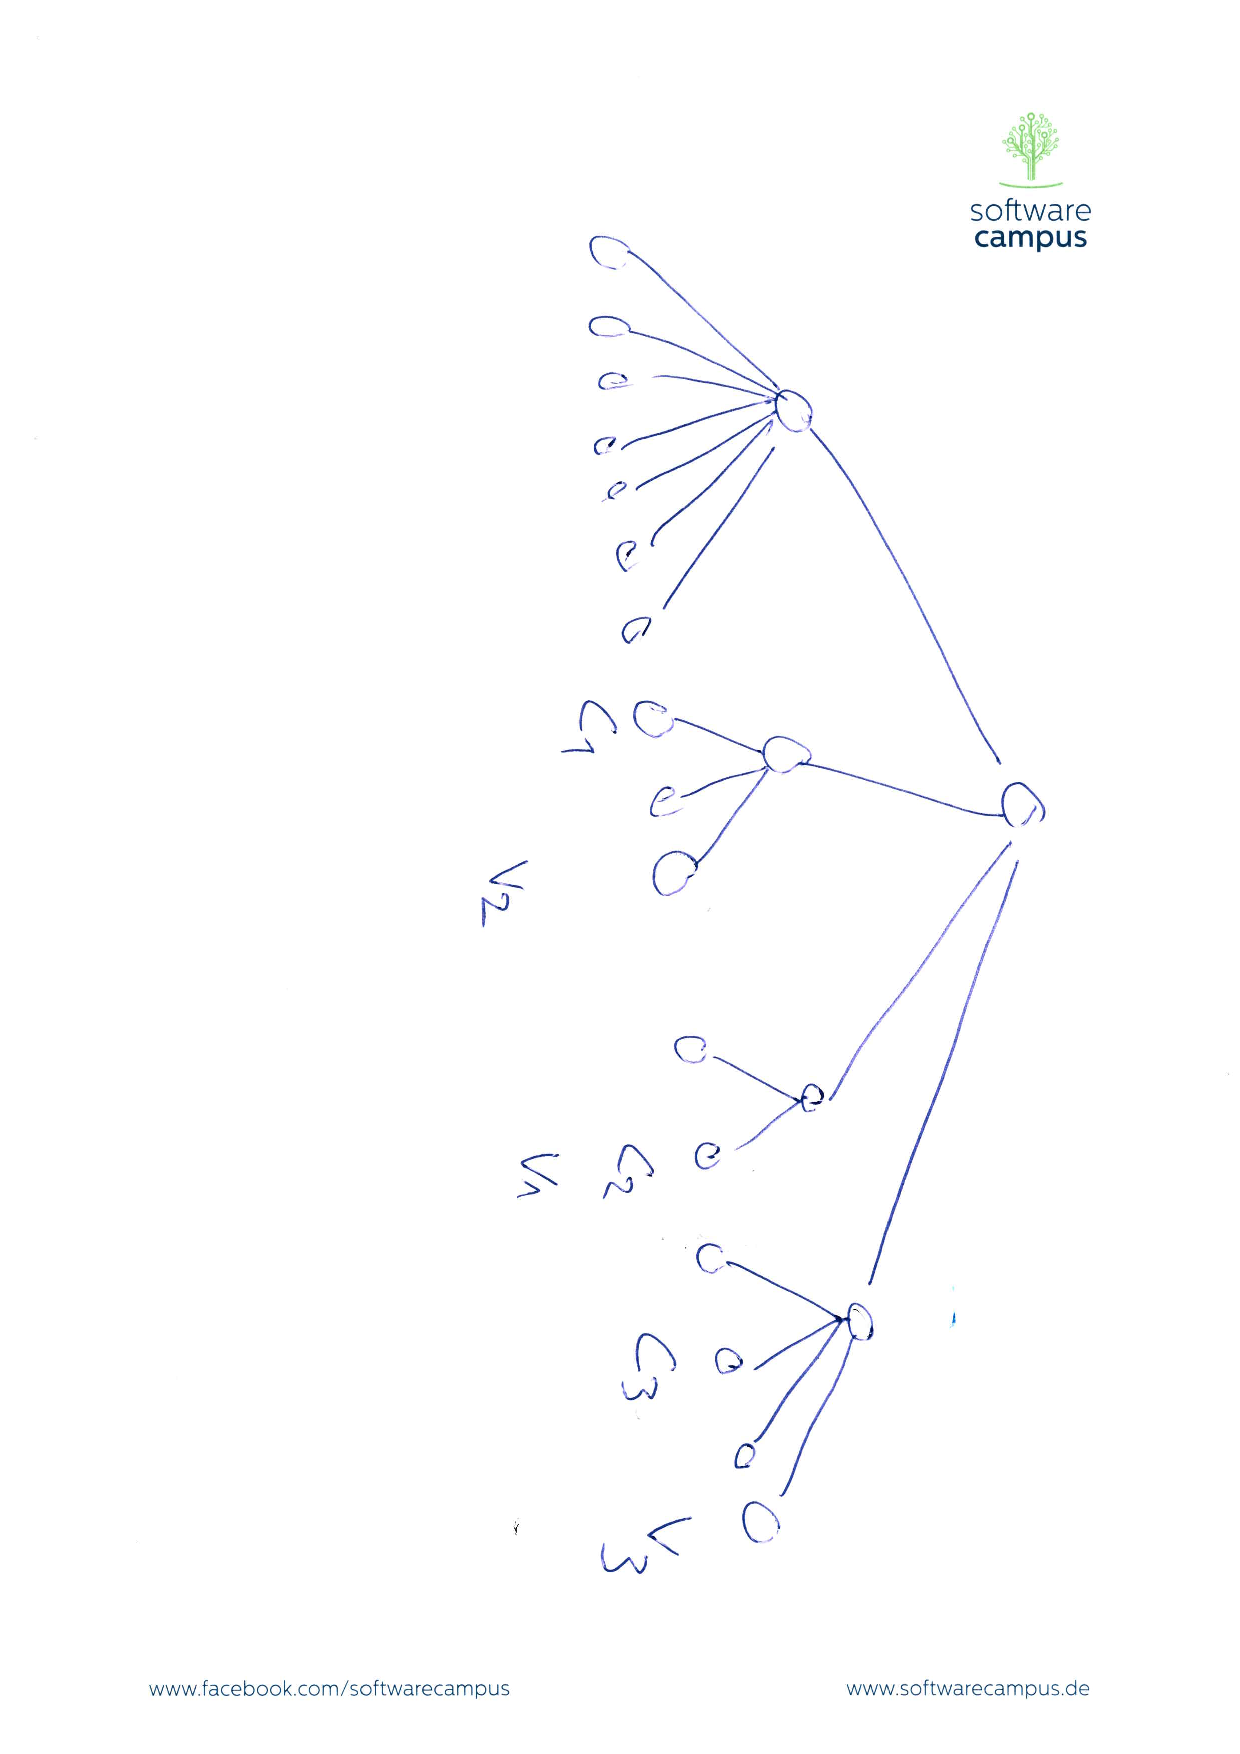
\includegraphics[angle=90,origin=c, height=7cm]{figs/model_fig_skteches/basic_problem}
\caption{solution for basic problem (green is pathes for transfer)}
\end{figure}

Throughout this section we will introduce different properties, to extend this
basic model. These properties can (and will) be combined to form more
challenging instances of $\Problem$.

%\begin{figure}[htbp]
%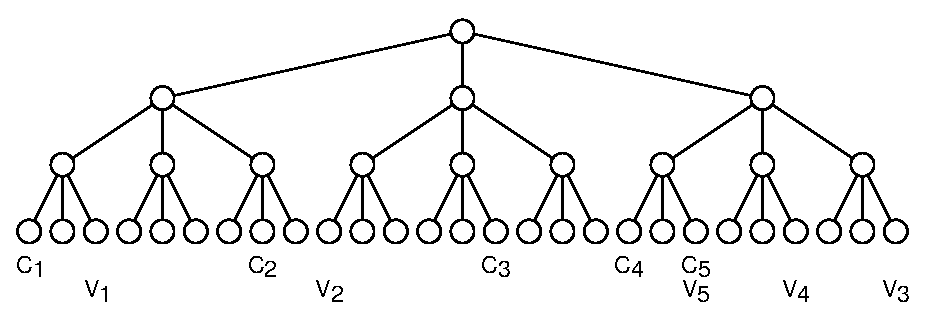
\includegraphics[width = \columnwidth]{figs/basic_scenario_3.eps}
%\caption{An example situation with 5 $\Chunk s$ and $\VM s$. Note that $c_5$
%and $v_5$ are on the same host.}
%\label{fig:model_clean}
%\end{figure}
%
%
%
%Figure~\ref{fig:model_clean} shows an example situation with $n = 5$. The goal
%of the $\Problem$  is to find an assignment of the $\VM s$ to the $\Chunk s$,
%which minimizes the overall bandwidth consumption of the job.
%
%We will now exemplarically examine an assignment of $\Chunk s$ to $\VM s$.
%Assume $c_1$ is assigned to $v_1$, $c2$ to $v2$, $c3$ to $v3$, $c4$ to $v4$
%and $c5$ to $v5$. Since $v_5$ runs on the same host, which contains $c_5$,
%transfering $c_5$ to $v_5$ will consume no bandwidth on the physical links.
%Hence we assume the overall bandwidth costs of the transfer to be $0$. The
%distrance between $v_1$ and $c_1$ is $2$ hops. Hence the transfer of the
%$\Chunk$ to the $\VM$ will consume bandwidth on two links. As a result, the
%overall bandwidth costs is $2 \cdot b_t$, where $b_t$ is the bandwidth
%neccessary for the transfer of a $\Chunk$. $v_4$ is $4$ hops away from $c_4$,
%which results in a total cost of $4 \cdot b_t$. Since the hop distance between
%$v_2$ and $c_2$ is 6, the costs for transferring the $\Chunk$ is $6 \cdot
%b_t$. The same holds for $v_3$ and $c_3$. The overall bandwidth consumption of
%the assignment is hence $18 \cdot b_t$.
%
%This is not an optimal solution for the $\Problem$. To show this, we will
%inspect a similar mapping. The only difference in the optimal mapping, is that
%$v_3$ is assigned to $c_2$ and $v_2$ is assigned to $c_3$. The bandwidth costs
%for transfering $c_2$ to it's assigned $\VM$ do not change, since $v_3$ is
%still $6$ hops away. $c_3$ however is now only $4$ hops away from its assigned
%$\VM$, which results in an overall bandwidth consumption of $16 \cdot b_t$.

\subsection{Communication Costs - $cv$}

\carlo{TODO: new symbol?}

This model extension assumes, that each VM  $\VirtualNode_i \in \VirtualNodes$
has to communicate with each other VM $\VirtualNode_{j \neq i} \in
\VirtualNodes$. Hence, the virtual cluster, which is to be embedded on the
physical substrate no longer consists only of a set of VMs, but is extended by a
set of virtual edges $\VirtualEdges : \VirtualNodes \times \VirtualNodes$.
Similar to the transfer of the chunks to the VMs, these edges have to be mapped
to a path in the host graph, which connects the locations to which the two VMs
are mapped. For the sake of simplicity we assume, that two VMs which communicate
inflict bandwidth cost of $\CostCom$ on each link of the path, which they use
for their communication.

\begin{figure}

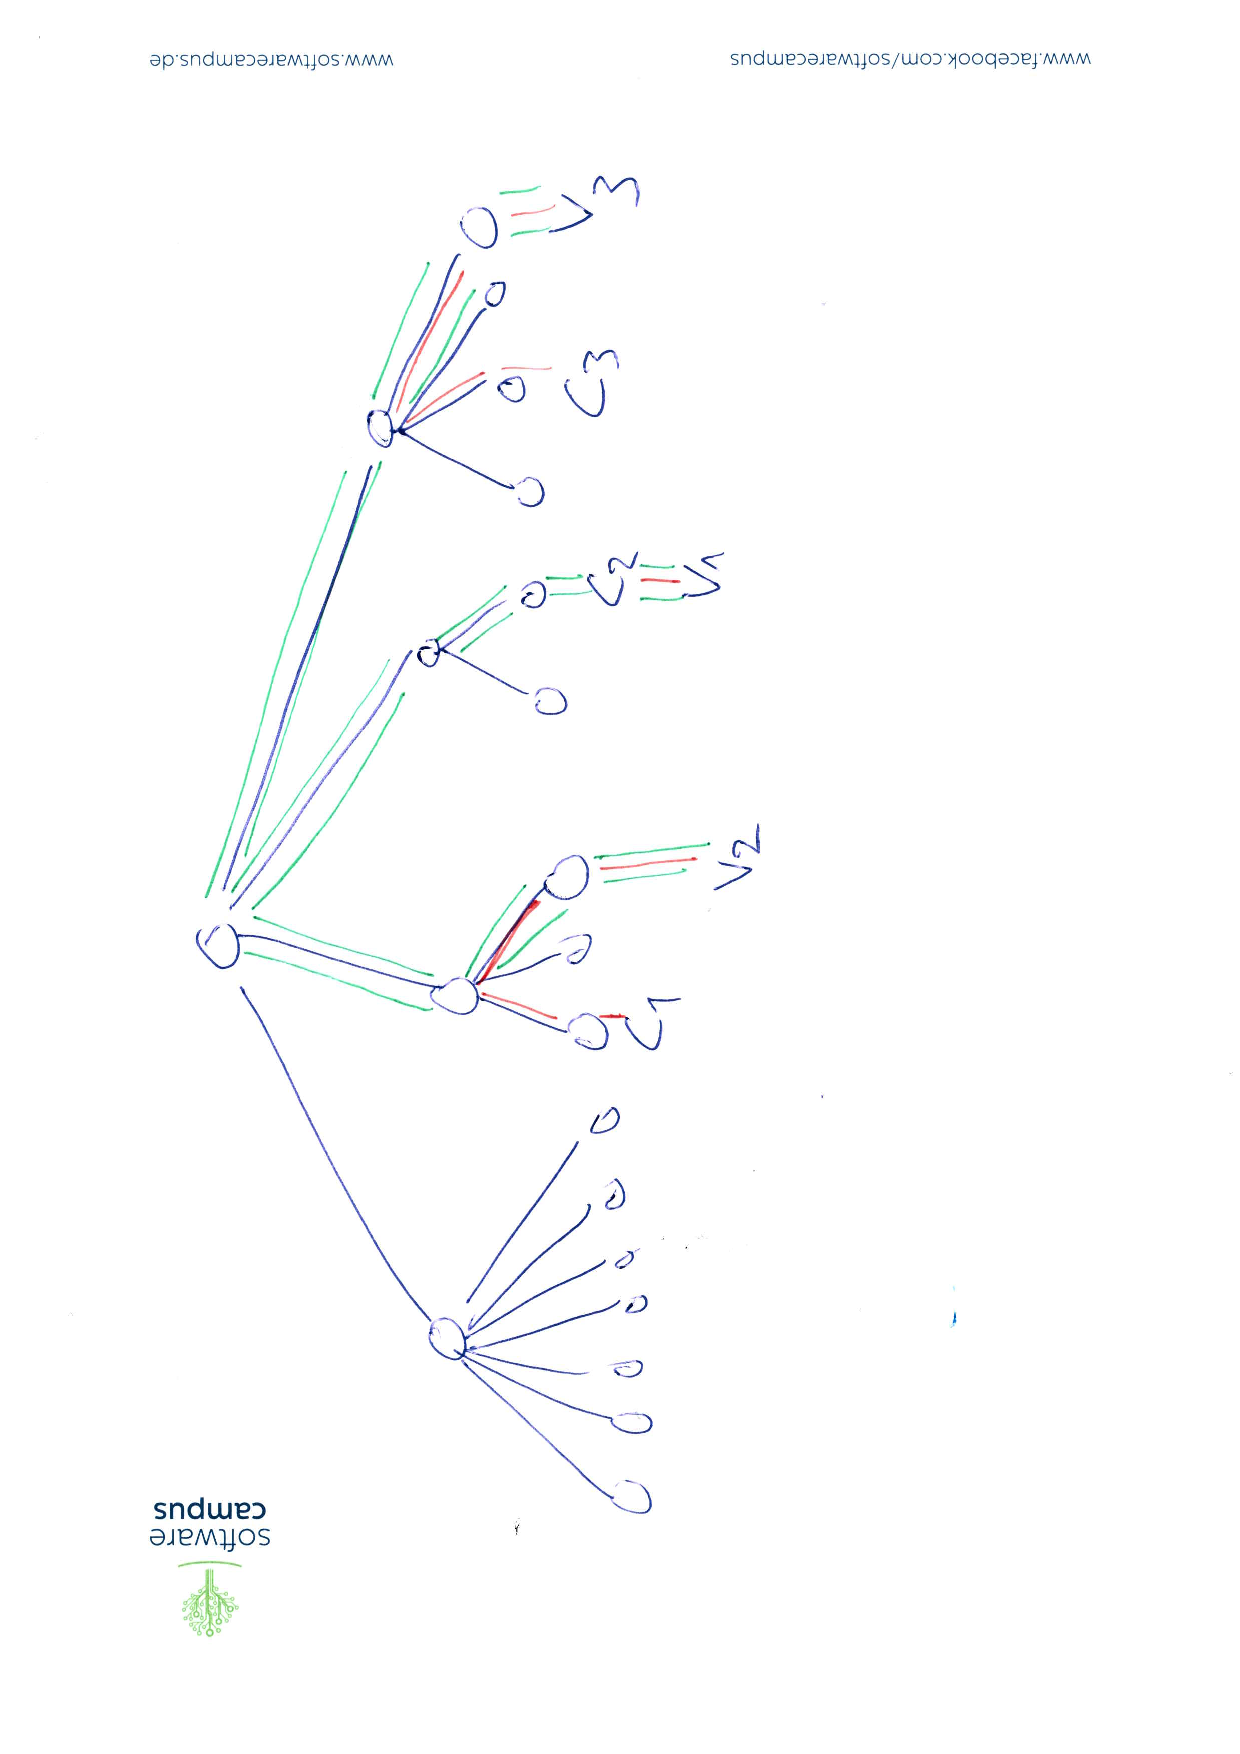
\includegraphics[angle=270,origin=c, height=7cm]{figs/model_fig_skteches/cv}
\caption{solution for problem with cv}
\end{figure}

%So
%far our model accounted bandwidth which is consumed to transfer data from it's
%location in the physical topology to the $\VM$ which will process it. However,
%due to the nature of distributed jobs, the $\VM s$ will also comunicate with
%each other. While we denoted the costs of transfering a chunk over a (1-hop)
%link with $b_t$, we will refer to the bandwidth costs of transfering data
%between a pair of $\VM s$ with $b_c$.


\subsection{Redundant Chunks - $r$}

This property specifies that, instead of having a single chunk $\Chunk_j$, we
have $\RedundancyFactor$ redundant copies of each chunk
$\Chunk_{j_1},\dots,\Chunk_{j_\RedundancyFactor}  \in \Chunks$. These copies are
entirely equal, and only one instance of a specific chunk type (e.g.
$\Chunk_{j_2}$) has to be read by one VM $\VirtualNode_j \in \VirtualNodes$.
Note that we assume chunks to be atomic - they cannot be read from two different
locations, requiering only $\CostTrans / 2$  bandwidth.

\begin{figure}

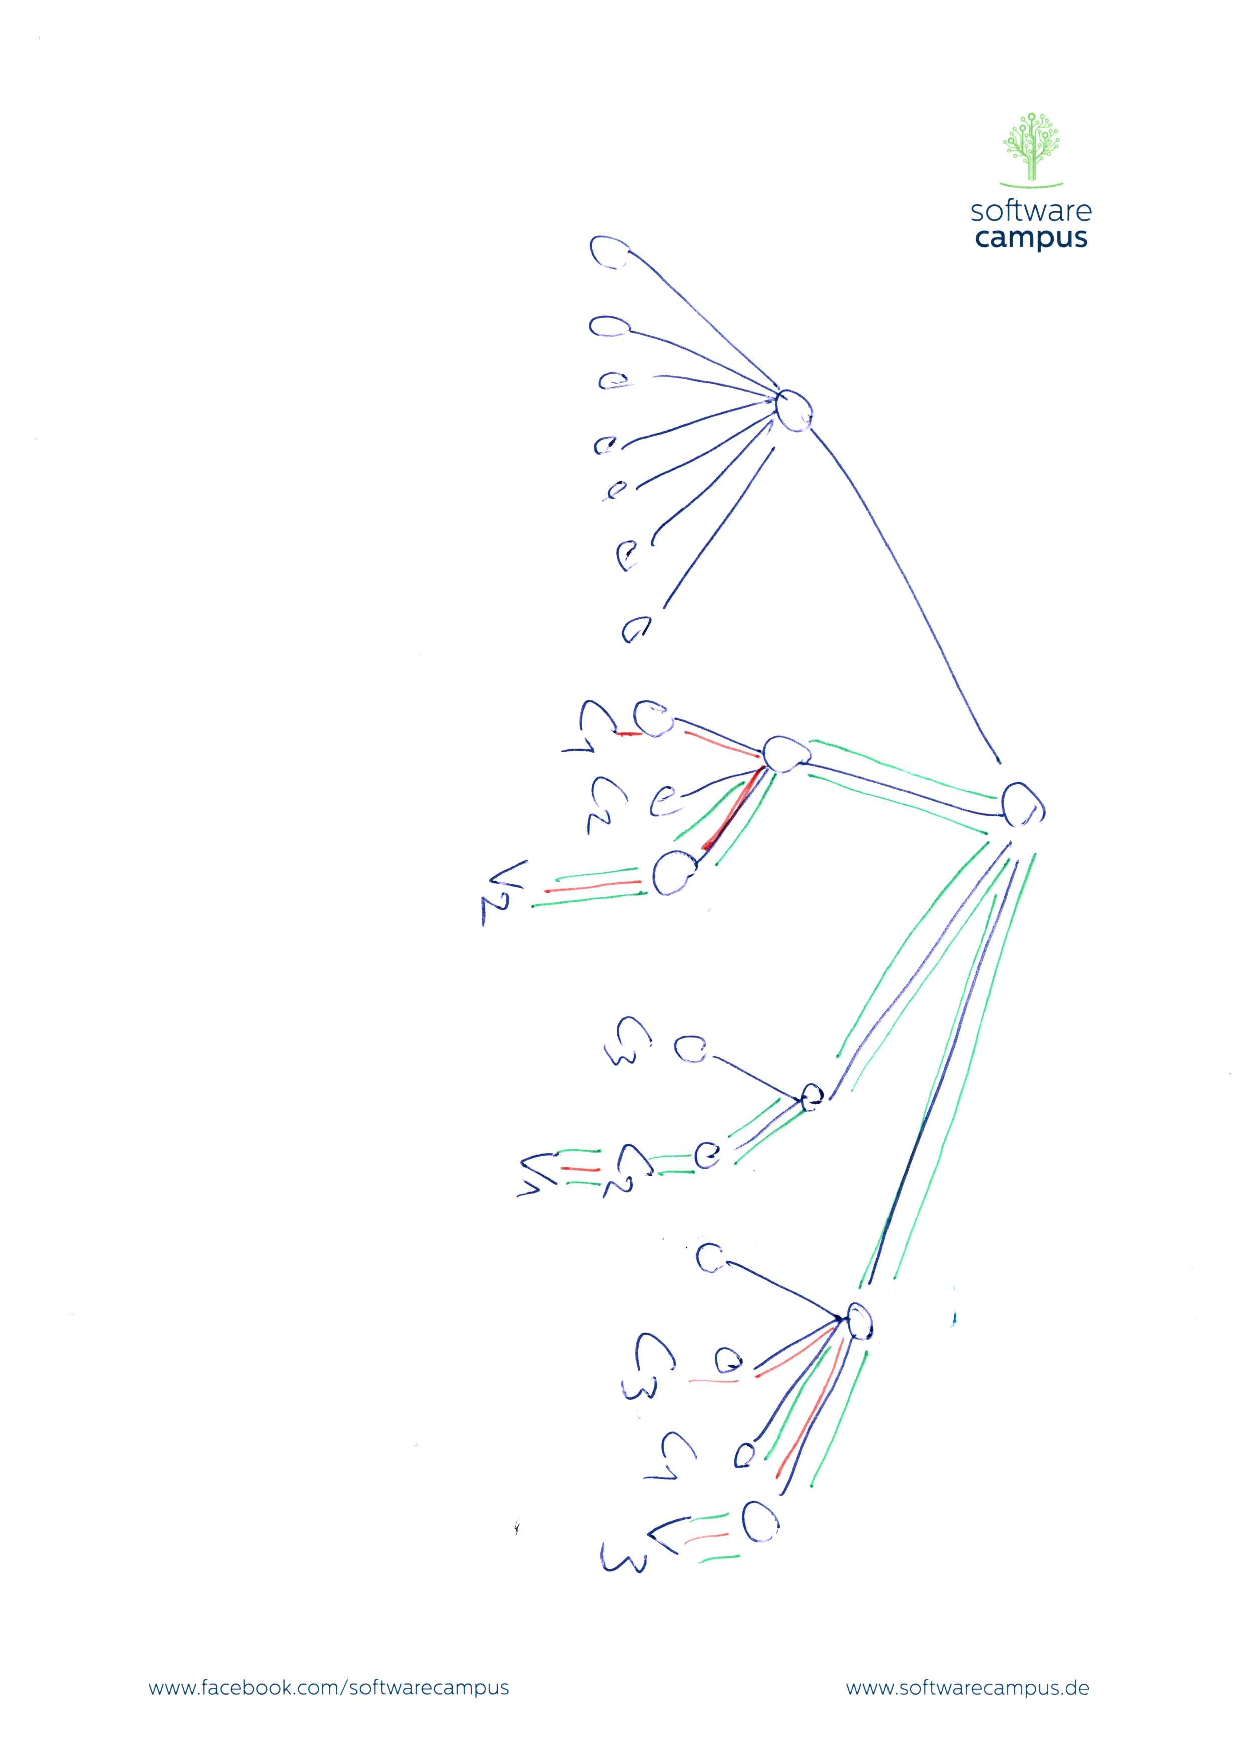
\includegraphics[angle=90,origin=c, height=7cm]{figs/model_fig_skteches/r_cv}
\caption{solution for problem with r}
\end{figure}




\subsection{Multiple Chunks per VM - $ma$}

This extension increases the processing capacities of the VMs. Instead of the
basic 1:1 ratio of VMs and chunks, this extension allows a VM to process
$\MaFactor \in \mathbb{N}^+$ many chunks. We assume, that the data which has to
be transferred to the VM from the chunks cannot be aggregated, and $\Vms =
\ChunkTypes / \MaFactor$.

\begin{figure}

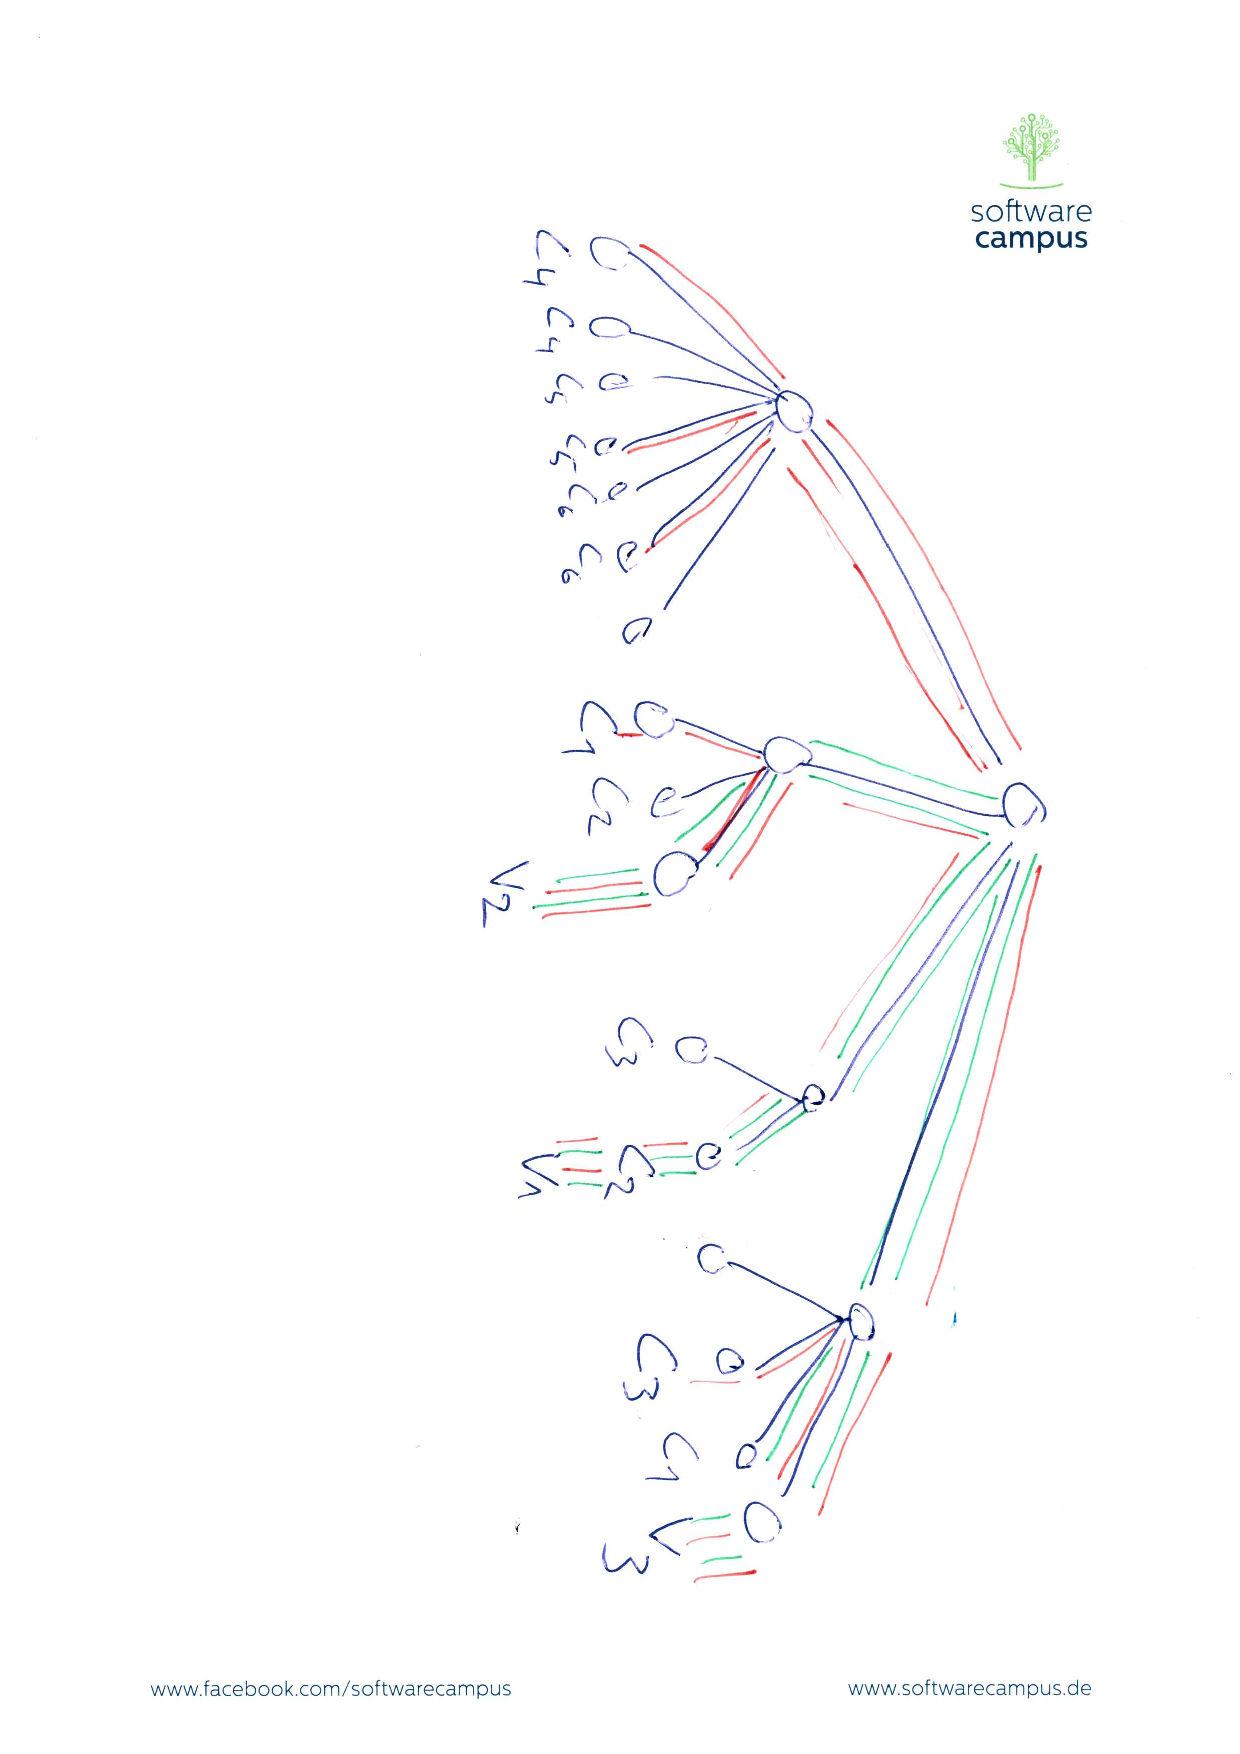
\includegraphics[angle=90,origin=c, height=7cm]{figs/model_fig_skteches/ma_r_cv}
\caption{soltion with ma}
\end{figure}

\subsection{Bandwidth Constraints - $bw$}

So far we only focussed on computing minimal bandwidth costs. However, in
reality the bandwidth which a single link can offer is limited. This model
extension limits the available bandwidth on each link $\SubstrateEdge_i \in
\SubstrateEdges$ in the host graph $\Tree$. We denote the capacity limitations
by $\Capacity : \SubstrateEdges \rightarrow \mathbb{R}$. The sum of all
bandwidth costs on this link, may never exeed it's capacity. Be aware that
this extension introduces infeasible instances.

\begin{figure}

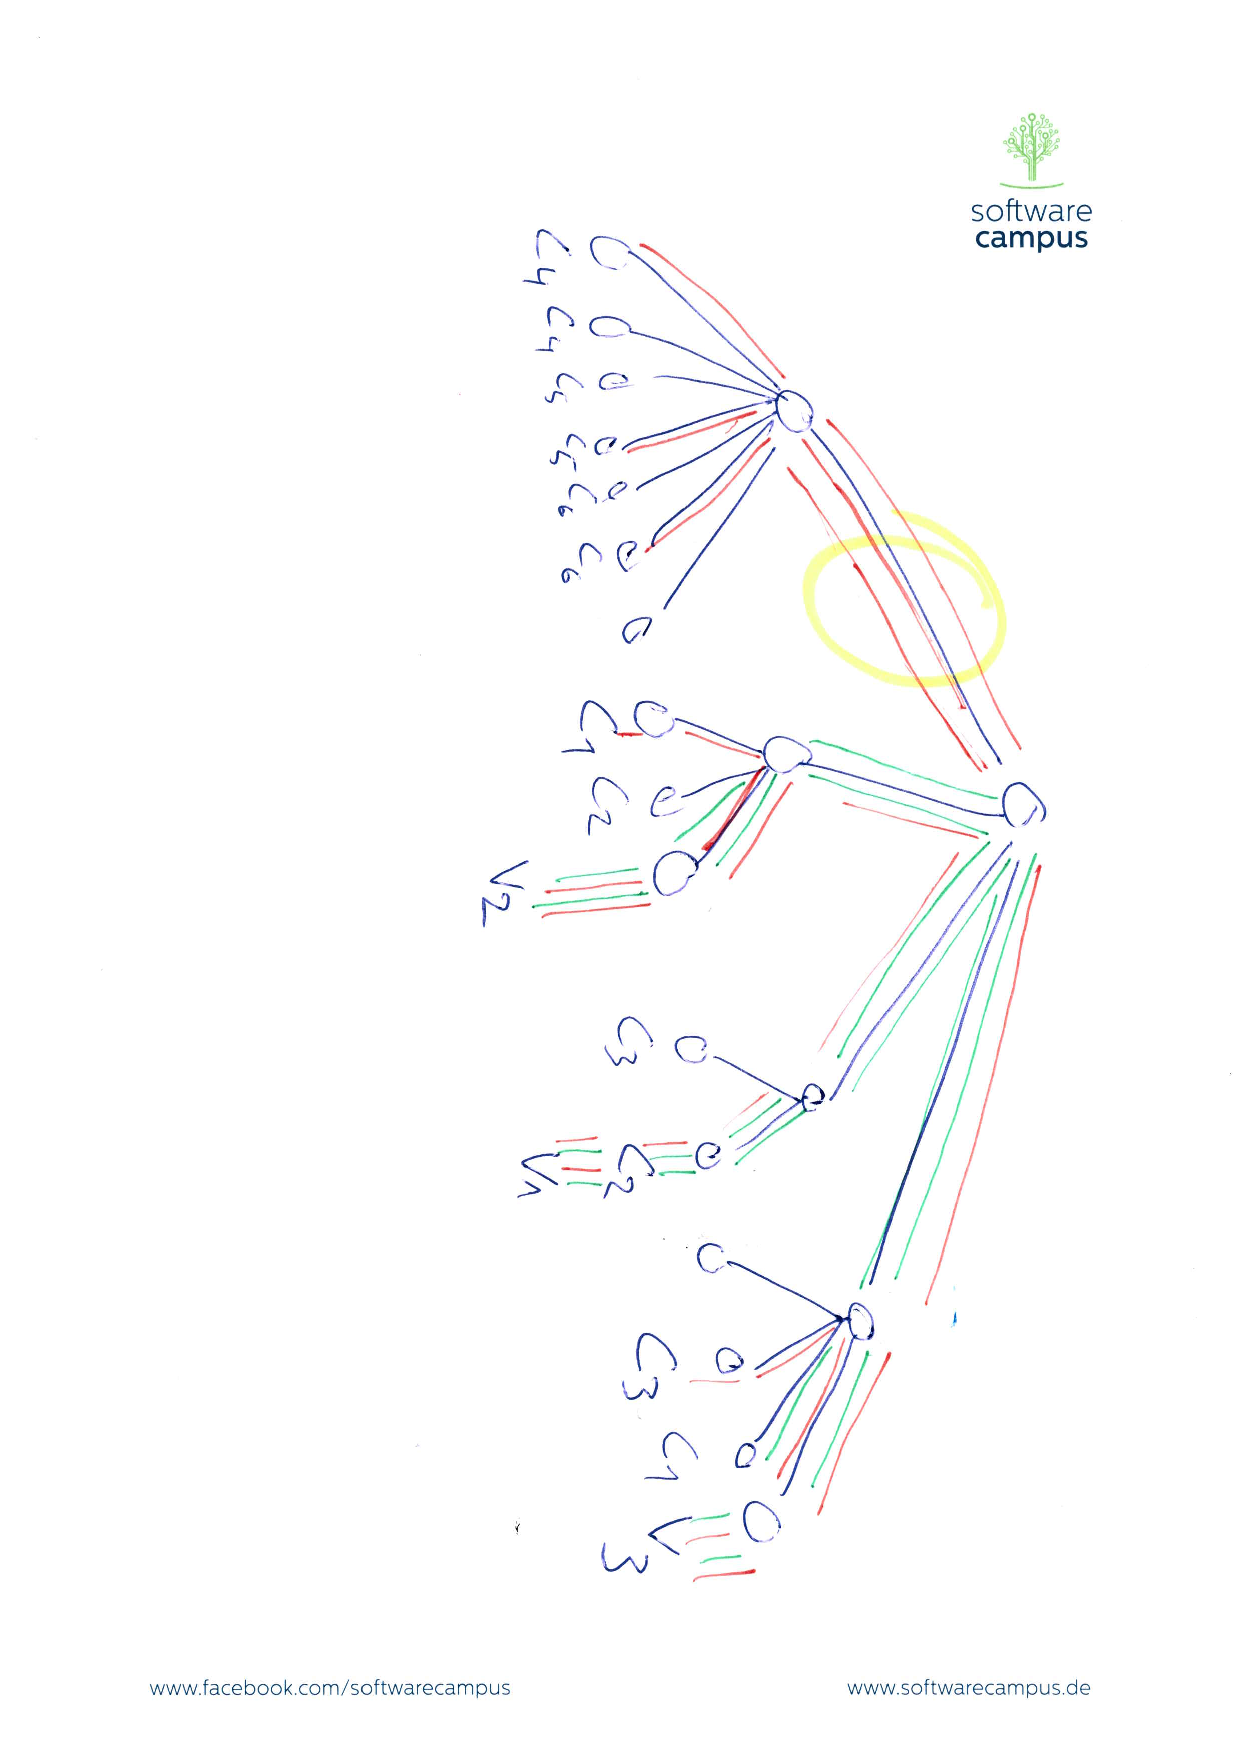
\includegraphics[angle=90,origin=c, height=7cm]{figs/model_fig_skteches/bw_ma_r_cv}
\caption{The bandwidth exceeds the capacity - independent of the chosen assignment}
\end{figure}
\subsection{Free VM Placement - $fp$}

The Free VM Placement property describes a variant of our simple model, where
the positions of the VMs are not given in the problem statement but are
rather chosen by the described strategy. Concretely, $\NodeMapping$ is no
longer given, but part of the optimization within $\Problem$. We assume that
each leaf can only host one VM.


\subsection{Summary of our results}

One day there will be a graph of all problems with arrows
corresponding to reductions and with partitioning to solution
approaches ((M)atching, (D)ynamic, (F)low, (N)p-hard).

\begin{enumerate}
\item basic problem - M
\item ma - M
\item r - M
\item cv - reduces to basic problem
\item bw - F
\item fp - solution of 0 cost
\item ma + r - M
\item  ma + bw - F
\item ma + cv - reduces to ma
\item ma + fp - D
\item r + bw - F
\item r + cv - reduces to r
\item r + fp - solution of 0 cost
\item bw + cv - reduces to bw
\item bw + fp - D
\item fp + cv - D
\item ma + r + bw - F
\item ma + r + cv - reduces to ma + r
\item ma + r + fp - N
\item ma + bw + cv - reduces to ma + bw
\item ma + bw + fp - D
\item ma + fp + cv - D
\item r + bw + cv - reduces to r + bw
\item r + cv + fp - N
\item r + bw + fp - solution of 0 cost
\item bw + cv + fp - D
\item ma + r + bw + cv - reduces to ma + r + bw
\item ma + r + bw + fp - N
\item ma + r + cv + fp - N
\item ma + fp + cv + bw - D
\item r + bw + cv + fp - N
\item ma + r + bw + cv + fp - N
\end{enumerate}


\begin{figure}[htbp]
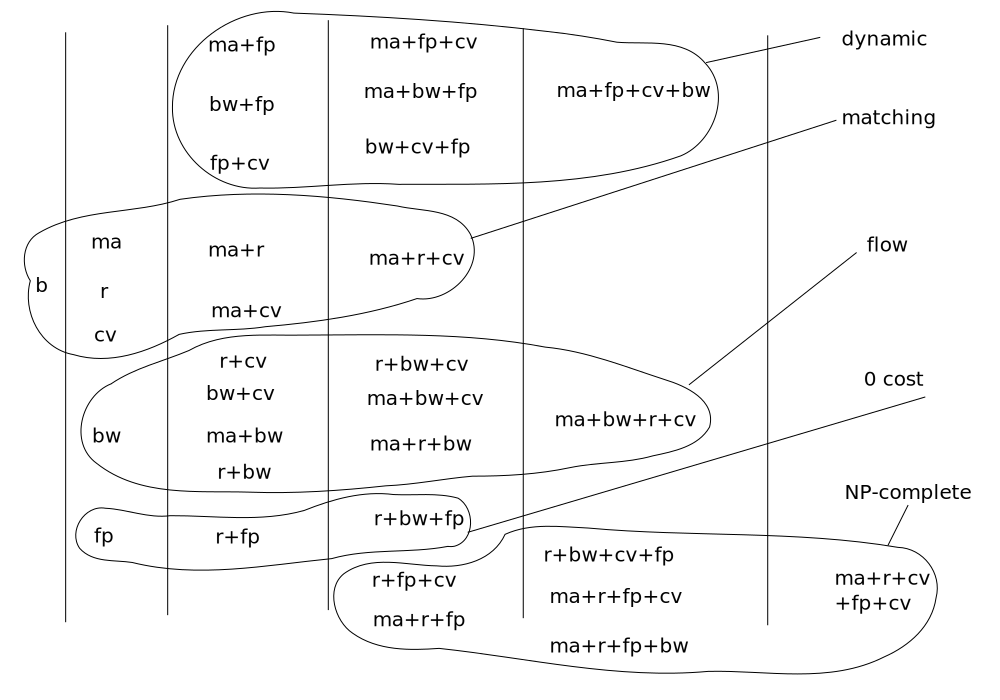
\includegraphics[width = \columnwidth]{figs/summary}
\caption{foo}
\label{fig:summary}
\end{figure}



%%%%%%%%%%%%%%%%%%%%%%%%%%%%%%%%%%%%%

\subsection{Matching based solutions} 

In the simplest version of $\Problem$, where all properties are absent, each VM 
is allready placed, the loactions of all chunks are known, and we have to 
compute an assignment of VMs to chunks, such that each VM is assigned to 
exactly one chunk, and each chunk is assigned to exactly one chunk. Hence we 
can transform each instance of $\Problem$ to a minimum weight perfect bipartite 
matching problem. One of the sets is formed by $\VirtualNodes$, the other by the 
set of chunks. A VM has an edge to each chunk. The costs of these edges are 
defined by the hop count between the VM and the chunk in the host graph. Each 
edge which is chosen for the solution of the matching problem, indicates that 
the chunk is assigned to the vm of the edge.

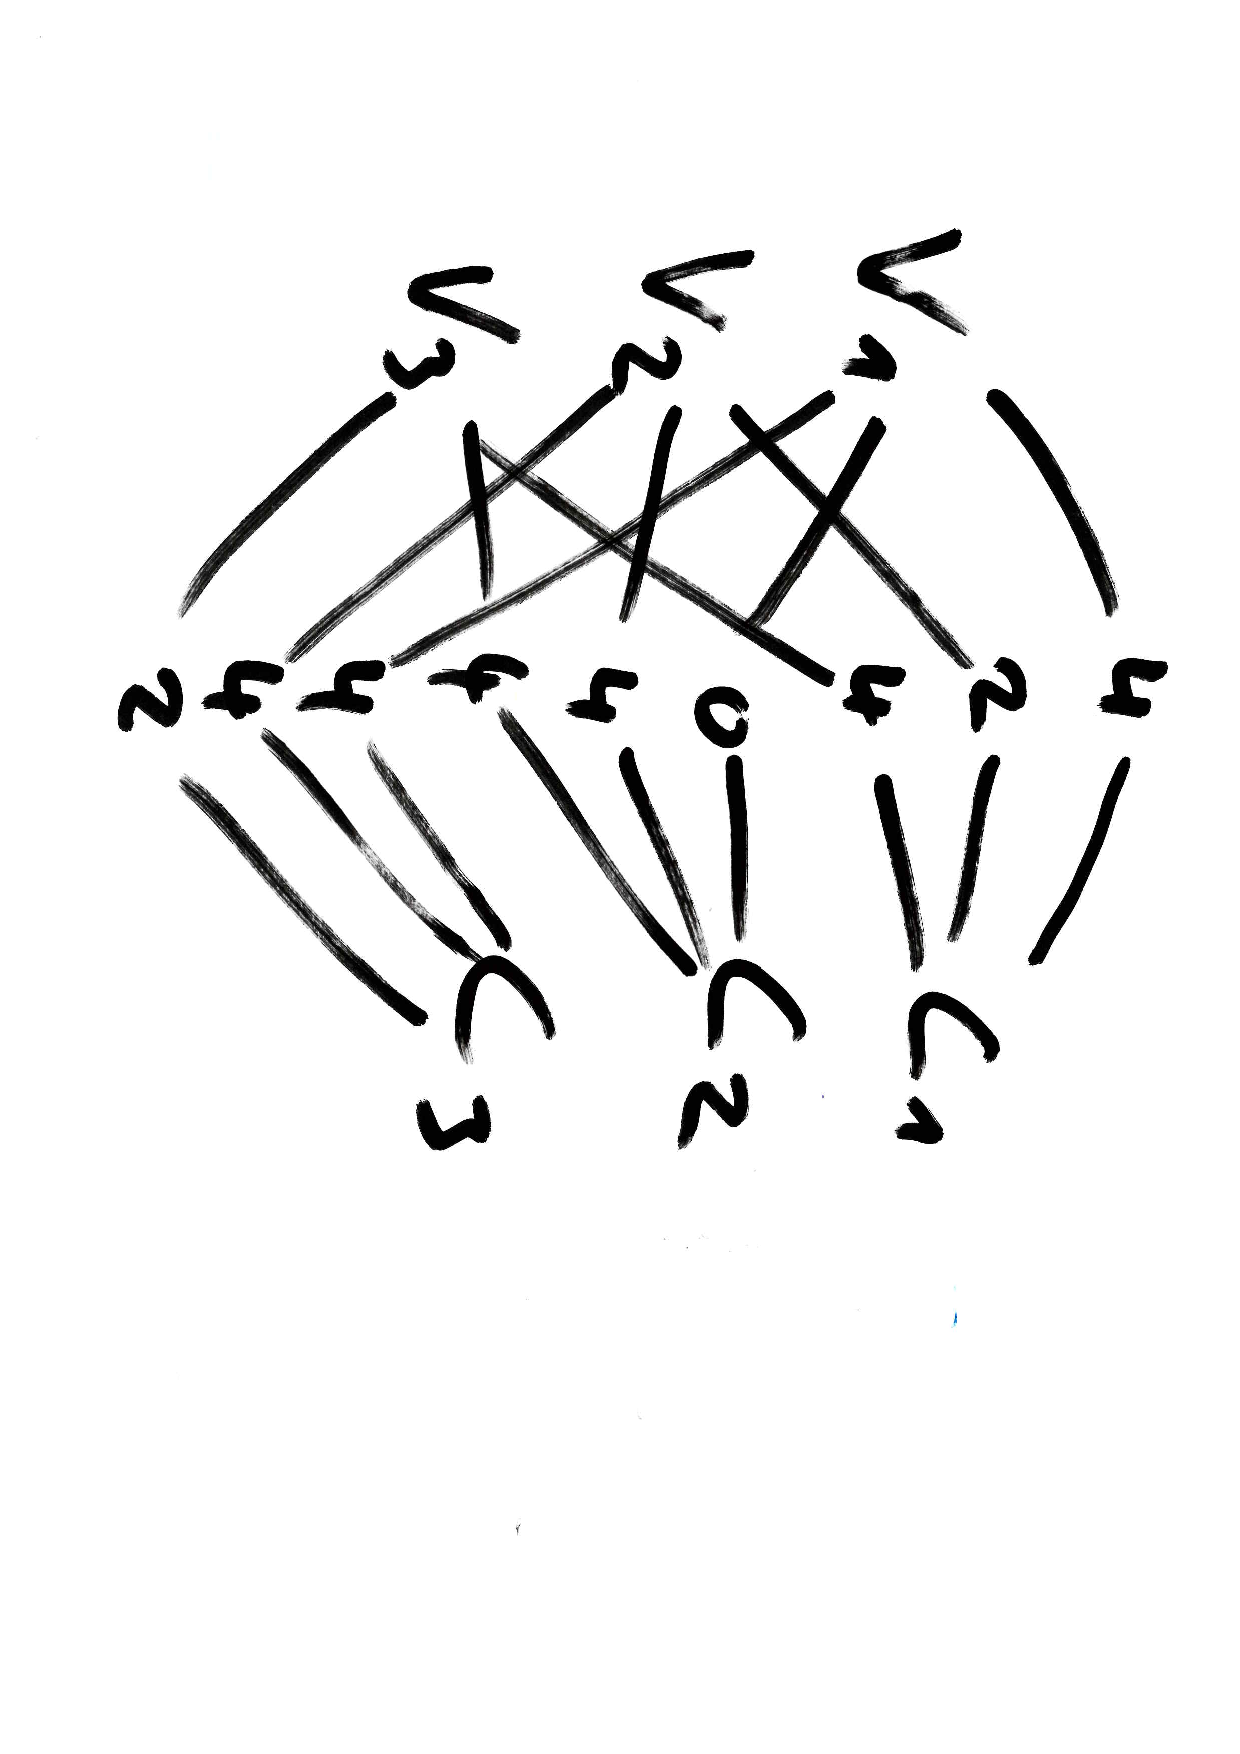
\includegraphics[angle=90,origin=c, 
height=7cm]{figs/model_fig_skteches/matching_basic}

This approach can also be used to solve instance of $\Problem$, which have the 
$ma$ or $r$ property - or even both. 
To Account for the $ma$ property, a single VM has to process exactly 
$\MaFactor$ VMs. Hence we can clone a VM to be represented by $\MaFactor$ Nodes.
In order to incorporate the different 
replicas of the chunks, we depict all copies of a given $\ChunkTypes$ in a 
single %$\ChunkType$ 
node. We connect each VM to all $\ChunkTypes$ using the 
lowest hop count to one of the copies as the weight.

Many algorithms solve the minimum weith perfect matching problem on bipartite 
graphs. The algorithms runtimes depend on  the number of nodes in the 
graph $n$, the number of edges in the graph $m$, and the largest magnitude of 
an edge weight $N$. An efficient algorithm is described by Gabow et al. in 
\cite{gabow_scaling_algorithm} and provides a runtime of $\mathcal{O}(n^{3/4} 
\cdot m \cdot \log n)$ which translates to $\mathcal{O}((\MaFactor \cdot \Vms + 
\ChunkTypes)^{3/4} \cdot  \MaFactor \cdot \Vms \cdot \ChunkTypes \cdot \log 
(2 \cdot h(\Tree)))$, where $h(T)$ denotes the height of the tree.

%\subsection{Dynamic programming solution}
Model:
\begin{itemize}
  \item We are given a tree $T$ with capacities $c_e$ on the edges
    (physical network)easured in number of edges)
  \item We are given $n$ chunks that are assigned to leaves of $T$ (at
    most one chunk to one leaf)
  \item Our task is to place $n$ virtual machines on leaves of $T$ (at
    most one virtual machine to one leaf)
  \item Virtual machines can be placed directly on empty leaves or on leaves with chunks
  \item Each chunk has to be transferred to a virtual machine (matching), and the
    cost inlined by that is equal to $b_1$ times distance between
    chunk and virtual machine measured by number of edges
  \item Each virtual machine has to communicate with each other
    virtual machine, and the cost inclined by that is equal to $b_2$
    times distance between each pair of virtual machines meas total cost
\end{itemize}

Let's start by transforming our tree to binary tree with arbitrary
depth. We also introduce weights on edges (either $0$ or $1$). The
strategy we use is to clone every vertex $|children(v)| - 2$ times,
placing subsequent clones as right son of the previous one and placing
subsequent children as left son of the clone. Last child is placed as
right son of last clone.

Let's begin designing our algorithm by writing recursive formula for
minimal cost inclined by placing virtual machines in leaves of a given
tree. Our approach is to evaluate this function using bottom-up
technique using auxilary array, which yields a dynamic programming
solution. To find actual placements of virtual machines in addition to
the cost, we traverse the array backwards, following the path of
minimas.

Keep in mind that number of virtual machines is equal to number of
chunks. However, our function $f$ will be defined by structural
induction on the tree and we will invalidate the property of having
the same number of chunks and virtual machines in a given subtree (which is true when
we look at whole tree).

Let's define $f$ in following way. First argument is a subtree (with
available informations like number of chunks in its leaves), and the
second argument is number of virtual machines that we decided to place
in the subtree (given as first parameter). To calculate optimum
placement of $x$ virtual machines in subtree $T$ ($f(T, x)$) we will
consider every possible split of number $x$ into two positive integer
values: $l$ and $r = x - l$. We will place $l$ virtual machines in
left subtree of $T$ and $r$ virtual machines in right subtree of
$T$. Having such information allow us to compute how much cost we
incline through edge $e_1$ (which connects left subtree of $T$ to root
of $T$) and edge $e_2$ (which connects right subtree of $T$ to root of
$T$). In a given recursive call we charge only those two edges, rest
of edges will be charged is subsequent calls.

Our cost function consists of two factors. First one, communication cost
between virtual machines is easy to compute. We know how many virtual
machines are in left subtree, how many are in right subtree and how
many are in whole tree outside of $T$. For each pair of virtual
machines, first of which is in left subtree and second of which is in
right subtree, we charge $b_2 \cdot (w(e_1) + w(e_2))$. For each pair
of virtual machines, first of which is in left subtree and second of
which is outside $T$, we charge $b_2 \cdot w(e_1)$. Right subtree case
is symmetrical. Second factor of our cost function is the cost of
transferring chunks to virtual machines. Let's call number of chunks
in left subtree as $c_l$ and number of chunks in right subtree as
$c_r$. To incline minimal cost we connect chunks in given subtree to
virtual machines in the same subtree. If we can no longer do that,
because $v_i < c_i (i \in \{l,r\})$, then we connect leftover chunks
to virtual machines in second subtree of $T$. If we can no longer do
that, we connect leftover chunks outside of $T$. This strategy is
optimal, because connecting any other way can be amended (TODO: need
better argument here), inclining lower cost. Connections inside either
left or right subtrees inclines cost $0$ to edges $e_1$ and
$e_2$. Connections between left and right subtree incline cost $b_1
\cdot (w(e_1) + w(e_2))$. Connections from either subtree to outside
of $T$ inclines either $b_1 \cdot w(e_1)$ or $b_2 \cdot
w(e_2)$. Finally, we can write down our formula for $f$:

$$ f(T, x) = min_{l \in \{0, \ldots, x\}} \{ f(T_l, l) + f(T_r, x - l)
+ TransferCost + ConnectionCost\} $$

where $TransferCost$ and $ConnectionCost$ are constants independent of
$l$, and are defined in paragraph above. One simplifying observation
is that to calculate $ConnectionCost$ we can just use the absolute
value of difference
between number of chunks and number of virtual machines in a given
subtree, without knowing which is bigger, because in our model if
there are some virtual machines left, we know that some chunks from
outside will use the same transfer as if we have excessive chunks in
the subtree.

Regarding base case we
trivially define leaf case as having cost $0$ if $x = 0$, cost $b_2
\cdot (n-1) + b_1\cdot n$ if there is no chunk in the leaf, cost $b_2 \cdot (n-1) +
b_1 \cdot (n-1)$ if there is a chunk in the leaf and $\infty$ otherwise.

Capacity constraints are preserved in such way that we put $f(T, x) =
\infty$ if either $e_1$ or $e_2$ transfer cost added to communication
cost exceedes its capacity. Doing so guarantees that this
(impossible) case can never be chosen as a minimum on higher levels of
recurrence calls (unless all other ways are impossible as well). 

When it comes to time complexity of described algorithm, we spend
certain amount of time in every of $2|T|$ vertices of binary
tree (2 is there because of binary transformation). This time can be
bound by iterating over splits of $n$ into two integers, times some
constant and we do it for every possible number of VMs from $0$ to $n$. Therefore, resulting running time is $O(Nn^2)$.



%%%%%%%%%%%%%%%%%%%%%%%%%%%%%%%%%%%%%
\section{NP-Hardness results}

We have seen that even problems with multiple dimensions of
flexibility can be solved in polynomial time. We presented dynamic programming-based solution for
jointly optimization of flexible node placement, assigning multiple
chunks to the same VM, communication among VMs, even under capacity
constraints ($\FP+\MA+\CC+\BW$). We were able to produce solution for optimizing replica selection,
multiple assignment, VM communication, under capacity constraints in
scenario where VMs are already spawned in certain nodes ($\RS+\MA+\CC+\BW$).



This section now points out fundamental
limitations in terms of computational tractability. In particular, we
will show that problems become NP-hard if multiple replicas have to be
assigned to a node ($\FP+\RS+\MA$ is proved NP-hard in
Section~\ref{ssec:fprsma}) or if inter-connects have to be established
($\FP+\RS+\CC$ is proved NP-hard in Section~\ref{ssec:fprscc}); both
results hold even in uncapacitated networks, and even in trees
consisting of two levels only (e.g., in a
datacenter \emph{pod}). Hardness of those problem variants will result
in hardness of 4 other variants -- see generalization graph below.


\begin{figure}[htbp]
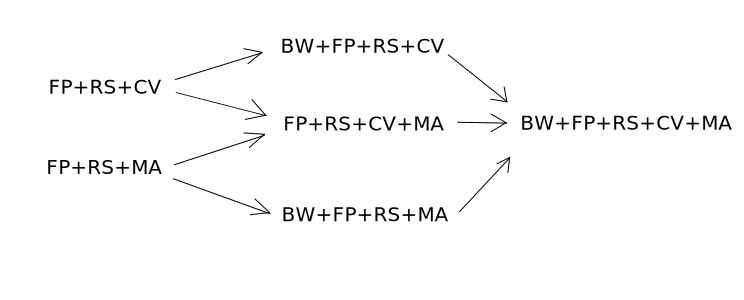
\includegraphics[width = \columnwidth]{figs/np-hierarchy}
\end{figure}



\subsection{Introduction to 3D Perfect Matching}

We start by introducing the NP-complete problem of 3D Perfect Matching
that will serve as problem we reduce from in both proofs. This problem
can be seen as a generalization of bipartite matchings to 3-uniform
hypergraphs, henceforth called $\TDM$.~\cite{3dmatch}

$\TDM$ is defined as follows. We are given three finite and disjoint
sets $X$, $Y$, and $Z$ of cardinality $k$, as well as a subset of triples $T\subset
X \times Y \times Z$.  Set $M \subseteq T$ is a 3-dimensional matching
if and only if, for any two distinct triples $(x_1, y_1, z_1) \in M$
and $(x_2, y_2, z_2) \in M$, it holds that $x_1\neq x_2$, $y_1\neq
y_2$, and $z_1\neq z_2$. Our goal is to decide if we can construct
such $M \subseteq T$ that is perfect, which means that it covers all
elements of $X \times Y \times Z$.

TODO: cite Karp on result of NP-completeness
TODO: image like this: \url{https://upload.wikimedia.org/wikipedia/commons/thumb/5/50/3-dimensional-matching.svg/240px-3-dimensional-matching.svg.png}

\subsection{Multi-Assignments are hard ($\FP+\RS+\MA$)}\label{ssec:fprsma}

Here we will present high-level ideas about encoding $\TDM$ as
 $\FP+\RS+\MA$ instance:

 \begin{itemize} \item For every element of universe $X\cup Y\cup
 Z$, we create chunk type. Processing every chunk corresponds to
 covering whole universe.

 \item We will encode each tripple as $3$ leaves that are close to
 eachother. We place chunk replicas that correspond to elements of the
 tripple.

 \item Placement of VMs will correspond to choice of tripples. No
 matter in which leaf of the gadget the VM will spawn, we will take
 that tripple to solution. VM will process the chunk that it sits on
 top of, as well as chunks in other two leaves of the same gadget.
 
\item We will set threshold cost in such way that no VM process
any chunk outside of the gadget that VM sits in.
\end{itemize}

\textbf{Construction.}
Given an instance $I$ of $\TDM$, we construct an instance $I'$ of
$\FP+\RS+\MA$ as follows:
\begin{itemize}
\item (tree construction) We create a tree consisting of root vertex, and for each tripple
we create a gadget that we attach as direct child of the root. Each
gadget consists of four vertices, one being inner node and three
leaves (see figure below).
\item (chunks and chunk replicas) For each element in $X$, $Y$ and $Z$ we create chunk type
($3 \cdot k$ in total). For each tripple we create $3$ replicas of
chunks that correspond to elements of universe and we place those
replicas in leaves of corresponding gadget
\item (other properties) We set number of VMs to spawn to $k$; we set
$\CostTrans=1$; we set number of slots in each VM to $m=3$; we set
$\Thr=2 \cdot 2 \cdot k$
\end{itemize}

FIXME: The construction is illustrated in Figure~\ref{fig:fprsma}.

\textbf{Correctness.}
We can now show the computational hardness.
\begin{theorem}
$\FP+\RS+\MA$ is NP-hard.
\end{theorem}
\begin{proof}
Let $I$ be an instance of $\TDM$ and let $I'$ be an instance of
$\FP+\RS+\MA$ constructed as described above.
We prove that $I'$ has solution of cost $\leq \Thr$ if ($\Rightarrow$) and only if
($\Leftarrow$)
$I$ has a matching of size $k$.

($\Rightarrow$) Let us take a solution to $\TDM$. We spawn VM in every
gadget that corresponds to chosen triples. We match every chunk in a
gadget to machine in this gadget (only for chosen ones). Solution has
cost exactly $\Thr$.

($\Leftarrow$) Let's take solution to $VC$ instance of cost $\leq \Thr$. We
chose triples that correspond to gadgets where were VMs. Everything
was processed, therefore every element of X,Y and Z is matched.
\end{proof}


\subsection{Inter-connects are hard ($\FP+\RS+\CC$) (reduction from 3D Perfect Matching)}\label{ssec:fprscc}


Next, we prove that the joint optimization of node placement and replica selection
is NP-hard if an inter-connect has to be established between virtual machines.
In our terminology, this is the $\FP+\RS+\CC$ problem.


\textbf{Construction.}
Given an instance of $\TDM$, we construct an instance of a
$\FP+\RS+\CC$ problem as follows. For each element
in the universe $X \cup Y \cup Z$, we construct a chunk; and for each
tripple $T_i$, we construct a gadget that contains
three replicas of chunks corresponding to the elements in the subset (those have 2 hops distance to eachother).
We connect the gadgets to the root, separating nodes from different tripples by 4 hops.

Concretely, let $I$ be an instance of $\TDM$. We will create an instance $I'$
for $\FP+\RS+\CC$ as follows:
\begin{itemize}
\item We set the access cost $\CostTrans$ to a chunk replica to a high value $W$. This will force
nodes to be collocated with the replica.
(For now, we can assume that $W=\infty$; a lower and sufficient bound will be given
in the appendix.)
\item The communication cost in the inter-connect is set to $\CostCom = 1$.
\item The number of nodes (virtual machines) is $\Vms = 3 \cdot k$. TODO: check again
\item We use a threshold $\Thr =  3 \cdot k + 3 \cdot 3 \cdot 2 \cdot (k - 1)$. TODO: check again
\end{itemize}

We construct a height-2 substrate tree
as follows. For each $T_i$ we construct a gadget
consisting of an inner node (a router) and three leaves. Every gadget
contains three chunks, corresponding to the elements of $T_i$.

FIXME: The construction is illustrated in Figure~\ref{fig:fprscc}.

\textbf{Proof of correctness.}
Intuitively, in order to minimize embedding costs,
nodes should be placed on near-by replicas. We use the following
helper lemma.
\begin{lemma}\label{lemma:helper}
In every valid solution $\Sol$ of $I'$ of cost $\leq \Thr$, each gadget
falls in one of two categories:
$k$ gadgets have exactly
$3$ nodes, and $n-k$ gadgets remain empty.
\end{lemma}
\begin{proof}
TODO: use exact cover property here to reason about feasibility

Since $W=\infty$, nodes will always be placed
directly on chunks (the access network cost is zero).
Moreover, since
$\Sol$ is valid, $3 \cdot k$ nodes are mapped
directly to the different chunk locations.
Now, consider any pair of nodes communicating over the
inter-connect; due to our construction, the communication cost
for each such pair is either
2 hops (if they belong to the same gadget) or 4 hops (if they belong
to different gadgets).
The lemma then follows from the observation that $\Thr$
is chosen such that it is never possible to distribute nodes
among more than $k$ gadgets, and that it is always strictly better to
have exactly 0 or 3 nodes per gadget, than any alternative distribution.
\end{proof}

\begin{theorem}
$\FP+\RS+\CC$ is NP-hard.
\end{theorem}
\begin{proof}
Let $I$ be an instance of $\TDM$ and let $I'$ be an instance of
$\FP+\RS+\CC$ constructed as described above.
We prove that $I'$ has solution of cost $\leq \Thr$ if ($\Rightarrow$) and only if
($\Leftarrow$)
$I$ has a solution.

($\Rightarrow$) In order to compute a solution
for $I'$ given a solution for $I$, we proceed as follows.
Given a covering set of tripples $S = \{T_1, T_2, \ldots, T_k\}$, we place three nodes in each gadget that
corresponds to every tripple of $S$. Chunks are matched to VMs that sit on top of them.

The solution has the following cost:
(1) the communication cost inside a gadget is $2 \cdot {3 \choose 2}$,
  as every pair contributes two hops;
  (2) the communication cost from each gadget to all other gadgets is $4
  \cdot 3 \cdot 3 \cdot (k - 1) / 2$, where the factor $2$ is
  for the
  communication over $4$ hops, the factor $3$
  corresponds to the number of nodes per gadget, and
  $3 \cdot (k-1)$ is the number of nodes in remote gadgets;
  as we count each pair twice, we need to divide by two in the end.
Summing up over all $k$ gadgets, we get exactly $\Thr$.

($\Leftarrow$) Given a solution for $I'$,
we can exploit Lemma~\ref{lemma:helper} to construct a solution for $I$.
We know that in any solution of cost at most $\Thr$,
$k$ gadgets contain exactly 3 nodes. These gadgets correspond to a valid
3D Perfect Matching of size $k$: every
chunk and hence element in the $X \cup Y \cup Z$, is matched.
\end{proof}




%%%%%%%%%%%%%%%%%%%%%%%%%%%%%%%%%%%%%
\section{Related Work}\label{sec:relwork}

It is well-known~\cite{talk-about} that the network
can have a significant impact on cloud application
performance, and several solutions have been proposed
over the last years to provide more predictable
network guarantees, such as avoiding multi-tenancy
entirely (see e.g., Amazon's Compute Cluster), by providing relative max-min
per-flow or per-tenant fairness
guarantees~\cite{seawall,netshare,faircloud,elasticswitch}, or by
explicit bandwidth
reservations~\cite{gatekeeper,secondnet,oktopus, proteus, drl}.

Our work focuses on systems with strict performance guarantees,
and there exists a large body of literature
on the general virtual network embedding problem, see~\cite{alloc-survey} for a good survey.
We consider the virtual cluster abstraction proposed
in the Oktopus~\cite{oktopus} paper, and later also studied in
the Proteus~\cite{proteus} paper. However, both papers only present
heuristic algorithms for the virtual cluster embedding problem.
While on average and in our simulations Oktopus~\cite{oktopus} and
Proteus~\cite{proteus} find good embeddings with small footprints,
it is easy to see that the resulting resource footprint
can be arbitrarily bad compared to the optimal solution.
Oktopus can miss solutions where the virtual cluster
is embeddable on a single server, and Proteus can miss efficient embeddings
spanning more than one pod.

FIXME: data locality, matching, etc.

%%%%%%%%%%%%%%%%%%%%%%%%%%%%%%%%%%%%%
\section{Conclusion}\label{sec:conclusion}

FIXME

%%%%%%%%%%%%%%%%%%%%%%%%%%%%%%%%%%%%%
\section{Appendix}

%%%%%%%%%%%%%%%%%%%%%%%%%%%%%%%%%%%%%
\bibliographystyle{alpha}
\bibliography{references}

\end{document}
